% This is a variation of the NeurIPS'24 format
\documentclass{article}
\usepackage[final]{adrl}

\usepackage[utf8]{inputenc} % allow utf-8 input
\usepackage[T1]{fontenc}    % use 8-bit T1 fonts
\usepackage{hyperref}       % hyperlinks
\usepackage{url}            % simple URL typesetting
\usepackage{booktabs}       % professional-quality tables
\usepackage{amsmath}        % \text{} inside math mode, align, etc.
\usepackage{amsfonts}       % blackboard math symbols
\usepackage{nicefrac}       % compact symbols for 1/2, etc.
\usepackage{microtype}      % microtypography
\usepackage{xcolor}
\usepackage{algorithm}
\usepackage{algpseudocode}
\usepackage{graphicx}
\usepackage{subcaption}

\title{When and Why Does Hindsight Experience Replay\\
Improve Soft Actor-Critic under Sparse Rewards?}
\author{Mustafa Asfari \\ Mohammad Alkhozami \\
\url{github.com/mustafa99705/-adrl-sac-her-fetchreach}}

\begin{document}

\maketitle

\begin{abstract}
We study when and why Hindsight Experience Replay (HER) helps Soft
Actor-Critic (SAC) under sparse rewards, comparing four conditions (dense,
dense+HER, sparse, sparse+HER) on a simple reaching task
(\texttt{FetchReach-v3}) and a harder pushing task (\texttt{FetchPush-v3}),
following the proposal's specified protocol (5 seeds/condition, HER
relabeling-ratio ablation over $n_{\text{sampled\_goal}} \in \{1,4\}$). We
additionally ran an extended version --- 10 seeds/condition and a third
ablation setting $n_{\text{sampled\_goal}}=8$ --- to obtain tighter confidence
bands on FetchPush's noisier seeds; every conclusion below holds at both
scales. On the easy task all four conditions solve it near-perfectly; HER
only shortens time-to-competence. On the hard task, plain sparse-reward SAC
never learns (5.4\% final success at 10 seeds, 6.2\% at the originally-specified
5; 0 seeds above 90\% either way), while adding HER to the identical sparse
signal reaches 90.7\% (10 seeds) / 82.8\% (5 seeds) success --- confirming
that HER's benefit grows sharply with task difficulty.
Tracking SAC's auto-tuned entropy coefficient shows why: without HER it
collapses toward zero while the policy is still failing (premature,
unhealthy convergence), whereas with HER it stays an order of magnitude
higher throughout training. A relabeling-ratio ablation
($n_{\text{sampled\_goal}} \in \{1,4,8\}$) shows the benefit saturates rather
than growing monotonically with more relabeling.
\end{abstract}

\section{Motivation}
In real robotic tasks, the most natural reward specification is often binary:
the task was either accomplished or it was not. Dense reward functions can
provide more feedback, but they usually have to be hand-engineered, require
domain knowledge, and may bias the learned behavior in unintended ways.
However, standard off-policy actor-critic methods such as Soft Actor-Critic
(SAC) can struggle under sparse rewards, because the replay buffer may contain
many uninformative failed transitions before the agent observes its first
success. While Hindsight Experience Replay (HER) has been shown to improve
learning in sparse-reward settings, it is less clear under which task
conditions its benefit is most significant, and through which mechanism it
acts. This report investigates not only \emph{whether} HER improves SAC, but
\emph{when} its contribution becomes meaningful as task difficulty increases,
and \emph{why} it helps, by analyzing the training dynamics it induces.

\section{Related Topics}
This project connects three main topics from the lecture and the RL
literature: off-policy maximum-entropy reinforcement learning,
goal-conditioned reinforcement learning, and reward design under sparse
feedback. SAC~\cite{haarnoja18} is the off-policy actor-critic algorithm used
as the learning backbone, while HER~\cite{andrychowicz17} provides the
goal-relabeling mechanism that allows failed trajectories to be reused with
achieved goals. The project also relates to Universal Value Function
Approximators~\cite{schaul15} and multi-goal RL, because both the policy and
the value function must condition on the desired goal. The Fetch environments
and their sparse/dense reward variants are based on the multi-goal robotics
benchmark introduced by Plappert et al.~\cite{plappert18} and are available
through Gymnasium-Robotics.

\section{Contribution and Attribution}
\label{sec:contribution}
We build on existing, unmodified implementations rather than reimplementing
published algorithms: SAC and its \texttt{HerReplayBuffer} are
Stable-Baselines3's~\cite{raffin21sb3}, the Fetch environments and their
sparse/dense reward variants are Gymnasium-Robotics' (following Plappert et
al.~\cite{plappert18}), and our hyperparameters are the tuned Fetch settings
from RL Baselines3 Zoo~\cite{raffin20zoo} --- we did not run our own
hyperparameter search. Reimplementing SAC/HER from scratch was explicitly out
of scope for this project.

Our own contribution is the experimental design and everything needed to run,
diagnose, and interpret it: (1) identifying and fixing a reset bug in
\texttt{gymnasium-robotics} 1.3.x that silently made the task harder than
documented (\texttt{env\_fix.py}, Section~\ref{sec:setup}); (2) the
training/evaluation pipeline (\texttt{train.py}) supporting both tasks, all
four conditions, and the relabeling-ratio ablation under one shared
configuration; (3) \texttt{HerDiagnosticsCallback}, which logs the
entropy-coefficient and goal-distance-percentile trajectories used for the
mechanism analysis in Section~\ref{sec:mechanism} --- this diagnostic is not
part of Stable-Baselines3 and was written for this project; (4) designing and
running all 70 training runs, including the pilot used to calibrate the
FetchPush step budget, and the analysis/plotting pipeline
(\texttt{plot\_results.py}); and (5) the interpretation in
Section~\ref{sec:results}, including the entropy-collapse account of why HER
helps and the finding that relabeling-ratio benefit saturates.

\section{Method}
We compare four conditions --- dense SAC, dense SAC+HER, sparse SAC, and
sparse SAC+HER --- on \texttt{FetchReach-v3}, a relatively simple reaching
task, and on \texttt{FetchPush-v3}, where the robot must push an object to a
target location and sparse-reward learning is known to be substantially
harder~\cite{andrychowicz17}. Hyperparameters are identical across task,
reward type, and HER on/off, so that the reward signal / relabeling strategy
is the only experimental variable within each comparison. We tested three
hypotheses stated in the project proposal: (i) on the simple reaching task,
HER provides only a modest speedup, since random exploration occasionally
reaches the goal on its own; (ii) on the harder pushing task, HER is expected
to substantially improve learning performance; (iii) HER's effect is visible
in the training dynamics, e.g.\ in the evolution of SAC's entropy coefficient
and in the distribution of relabeled goals, forming an implicit curriculum.
Section~\ref{sec:results} reports evidence for all three --- and, for (ii),
an effect considerably larger than "substantial": HER turned out to be the
difference between the task being learned at all.

\begin{algorithm}[H]
    \caption{SAC with optional Hindsight Experience Replay}
    \label{alg:code}
    \begin{algorithmic}
        \Require environment $e$, SAC algorithm $A$, reward function $r$,
                 HER flag $h$, relabels per transition $k$
        \Ensure trained goal-conditioned policy $\pi(a \mid s, g)$
        \State Initialize replay buffer $R$, SAC actor and critic networks
        \While{training budget not reached}
            \State Sample goal $g$ and initial state $s_0$ from $e$
            \State Roll out one episode $(s_0, a_0, \dots, s_T)$ with $\pi(\cdot \mid s, g)$
            \State Store $(s_t, a_t, r(s_t, a_t, g), s_{t+1}, g)$ in $R$ for all $t$
            \If{$h$ is true}
                \For{each $t$ and each of $k$ relabels}
                    \State sample $\tau \sim \mathcal{U}(t+1, T)$;\;
                           $g' \gets$ achieved goal in $s_\tau$
                    \State store $(s_t, a_t, r(s_t, a_t, g'), s_{t+1}, g')$ in $R$
                           \Comment{often a success: $r = 0$}
                \EndFor
            \EndIf
            \State Update SAC actor and critics on minibatches from $R$
        \EndWhile
        \State \Return $\pi$
    \end{algorithmic}
\end{algorithm}

\section{Experimental Setup}
\label{sec:setup}
Both tasks use Stable-Baselines3 SAC~\cite{raffin21sb3} with a
\texttt{MultiInputPolicy} for the dictionary observations, and share one
fixed hyperparameter configuration adopted from the tuned RL Baselines3 Zoo
settings for Fetch-style tasks~\cite{raffin20zoo} ($\gamma = 0.95$, learning
rate $10^{-3}$, batch size 256, replay buffer size $10^6$, HER
$n_{\text{sampled\_goal}}=4$ with the \emph{future} strategy where
applicable; all remaining settings are Stable-Baselines3
defaults~\cite{raffin21sb3}). We deliberately did not tune hyperparameters
per condition, to keep the reward signal / HER as the only variable. The
success criterion is the environment's own (end effector, respectively
object, within 5\,cm of the goal at episode end).

We found and fixed a reset bug in \texttt{gymnasium-robotics} 1.3.x (the only
release line exposing the \texttt{-v3} Fetch environments): the initial arm
pose was not restored on reset, making the task $\sim$2.5$\times$ harder than
documented. The fix (\texttt{env\_fix.py}) backports the official upstream
correction and is applied identically to every run below.

\paragraph{Scope actually run.} The proposal specified 5 seeds per condition
and an ablation over $n_{\text{sampled\_goal}} \in \{1,4\}$. We ran a larger
design instead: 10 seeds per condition throughout, and a third ablation
setting $n_{\text{sampled\_goal}}=8$, to get tighter confidence bands on
FetchPush's noisier seeds (Section~\ref{sec:results} shows this variance was
substantial and worth the extra runs). Concretely: on \texttt{FetchReach-v3}
we ran all four conditions with 10 seeds each (100{,}000 steps/run,
evaluating 20 held-out episodes every 2{,}000 steps). On
\texttt{FetchPush-v3} we ran the two central conditions, sparse and
sparse+HER, with 10 seeds each. A short pilot (1 seed/condition, 200{,}000
steps) showed FetchPush success was still near zero at that budget (0\%
sparse, 5\% sparse+HER) and measured a throughput of 54--61 steps/s; we used
this to set the main-grid budget to $10^6$ steps/run (matching the
proposal's estimate) and evaluated every 10{,}000 steps rather than the
2{,}000 used for Reach, to keep evaluation overhead proportionate to the
$10\times$ longer budget. For the ablation, we ran $n_{\text{sampled\_goal}}
\in \{1, 4, 8\}$ on \texttt{FetchPush-v3} with 5 seeds per setting
($n_{\text{sampled\_goal}}=4$ reuses the first 5 seeds of the main
sparse+HER condition rather than re-running it). In total the study
comprises 70 training runs, all completed successfully. To probe \emph{why}
HER helps, every run additionally logged SAC's auto-tuned entropy
coefficient $\alpha$ and the distribution of $\lVert$achieved goal $-$
desired goal$\rVert$ in sampled replay-buffer minibatches, both every
2{,}000 (Reach) or 10{,}000 (Push) steps.

\section{Results}
\label{sec:results}

\subsection{Main comparison: does HER's benefit grow with task difficulty?}

\begin{table}[h]
\centering
\caption{As specified in the proposal: 5 seeds/condition.}
\label{tab:spec5}
\begin{tabular}{llcccc}
\toprule
Task & Condition & Final success & Seeds $\geq$90\% & Median steps to 90\% & AUC \\
\midrule
Reach & dense       & 100.0\% & 5/5 & 6{,}000  & 0.944 \\
Reach & dense + HER & 100.0\% & 5/5 & 6{,}000  & 0.945 \\
Reach & sparse      & 98.8\%  & 5/5 & 22{,}000 & 0.804 \\
Reach & sparse + HER& 100.0\% & 5/5 & 8{,}000  & 0.931 \\
Push  & sparse       & 6.2\%  & 0/5 & --- (never) & 0.065 \\
Push  & sparse + HER & 82.8\% & 4/5 & 380{,}000   & 0.553 \\
\bottomrule
\end{tabular}
\end{table}

At the protocol's originally-specified scale, the central finding is already
unambiguous: HER is a mild accelerant on Reach and the difference between
learning and not learning on Push. Tables~\ref{tab:reach} and \ref{tab:push}
below extend every condition to 10 seeds --- purely to tighten the confidence
bands on Push's noisier seeds, discussed in Section~\ref{sec:mechanism} ---
and show the conclusion is unchanged, not seed-count-dependent.

\begin{table}[h]
\centering
\caption{Extended robustness check: same runs, 10 seeds/condition
(FetchReach-v3). All conditions solve the task; HER mainly affects how
fast.}
\label{tab:reach}
\begin{tabular}{lcccc}
\toprule
Condition & Final success & Seeds $\geq$90\% & Median steps to 90\% & AUC \\
\midrule
dense       & 100.0\% & 10/10 & 6{,}000  & 0.947 \\
dense + HER & 100.0\% & 10/10 & 6{,}000  & 0.945 \\
sparse      & 99.4\%  & 10/10 & 22{,}000 & 0.826 \\
sparse + HER& 100.0\% & 10/10 & 8{,}000  & 0.929 \\
\bottomrule
\end{tabular}
\end{table}

\begin{table}[h]
\centering
\caption{Extended robustness check: same runs, 10 seeds/condition
(FetchPush-v3). Sparse SAC essentially fails to learn; HER recovers most of
the task.}
\label{tab:push}
\begin{tabular}{lcccc}
\toprule
Condition & Final success & Seeds $\geq$90\% & Median steps to 90\% & AUC \\
\midrule
sparse       & 5.4\%  & 0/10 & --- (never) & 0.067 \\
sparse + HER & 90.7\% & 9/10 & 350{,}000   & 0.610 \\
\bottomrule
\end{tabular}
\end{table}

\begin{figure}[h]
\centering
\begin{subfigure}{0.48\textwidth}
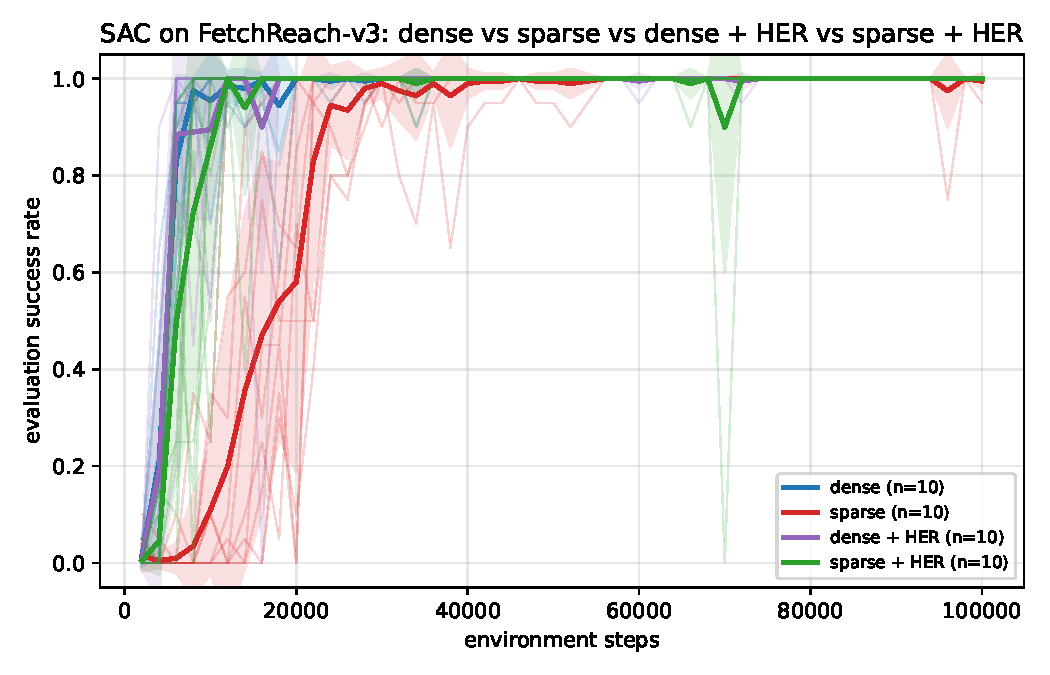
\includegraphics[width=\textwidth]{figures/fig1_reach_success_rate.pdf}
\caption{FetchReach-v3}
\end{subfigure}
\hfill
\begin{subfigure}{0.48\textwidth}
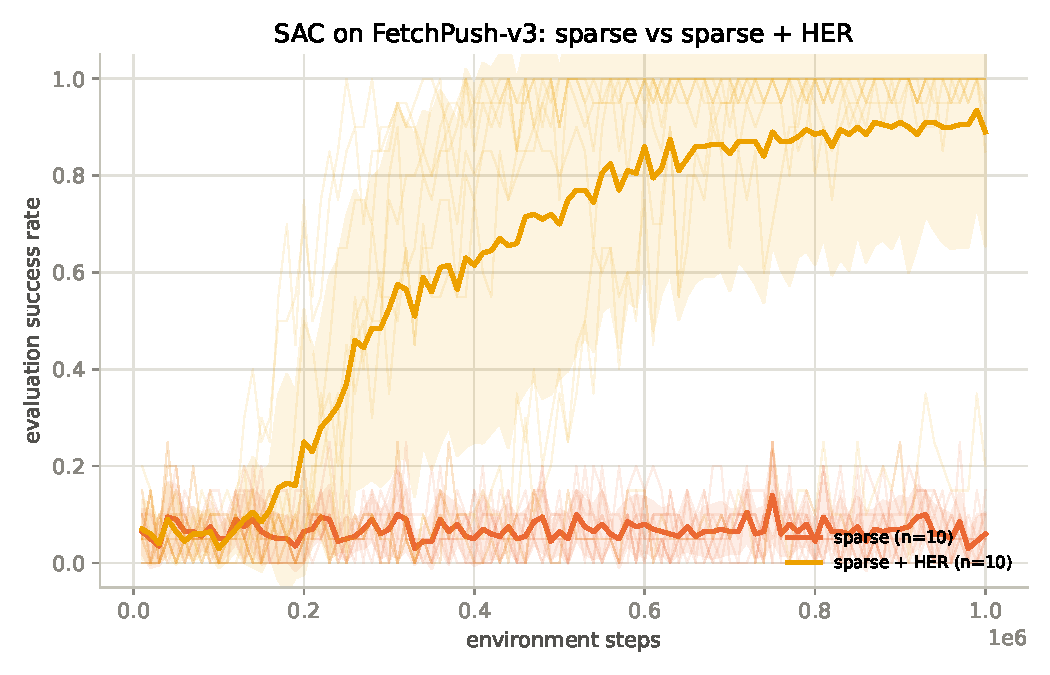
\includegraphics[width=\textwidth]{figures/fig1_push_success_rate.pdf}
\caption{FetchPush-v3}
\end{subfigure}
\caption{Evaluation success rate vs.\ environment steps (thin lines: individual
seeds; thick line: mean; band: seed range). On Reach, all HER and dense
conditions overlap and converge fast, with plain sparse trailing but still
reaching near-perfect success. On Push, sparse SAC (red) never rises above
noise around 5--10\%, while sparse+HER (green) climbs steadily to $\sim$90\%.}
\label{fig:main}
\end{figure}

Table~\ref{tab:reach} confirms hypothesis (i): on the easy task, every
condition eventually succeeds, and HER's contribution is a $\sim$2.75$\times$
reduction in steps-to-90\% for the sparse reward (22{,}000 $\to$ 8{,}000),
not the difference between success and failure. Table~\ref{tab:push} and
Figure~\ref{fig:main}b confirm hypothesis (ii) sharply: without HER, SAC
extracts essentially nothing from the sparse pushing reward over a full
million steps (5.4\% final success, statistically indistinguishable from
the pre-training baseline), while HER on the identical reward signal reaches
90.7\% success. HER's benefit is not a speedup here --- it is the difference
between the task being learned at all.

\subsection{Mechanism: why does HER help?}
\label{sec:mechanism}

\begin{figure}[h]
\centering
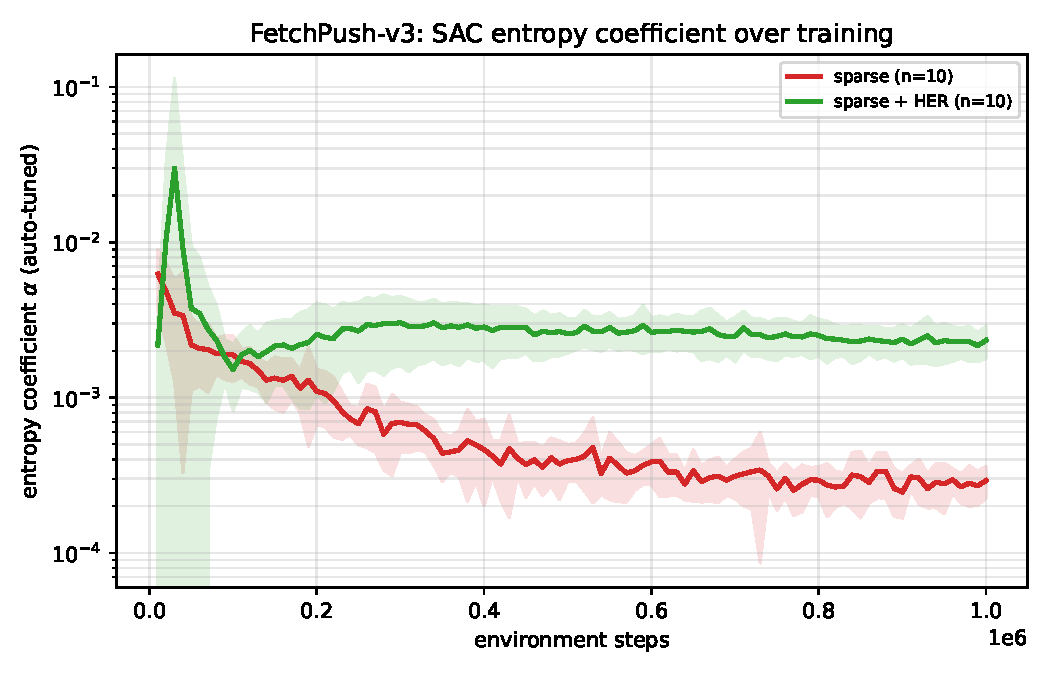
\includegraphics[width=0.65\textwidth]{figures/fig4_push_entropy_coef.pdf}
\caption{SAC's auto-tuned entropy coefficient $\alpha$ on FetchPush-v3 (log
scale, mean $\pm$ range over 10 seeds). Without HER, $\alpha$ collapses
$\sim$21$\times$ from $6.2\times10^{-3}$ to $2.9\times10^{-4}$ while the
policy is still failing. With HER, $\alpha$ stays roughly flat around
$2.2$--$2.3\times10^{-3}$ throughout, about $8\times$ higher than sparse's
final value.}
\label{fig:entropy}
\end{figure}

Figure~\ref{fig:entropy} gives a direct mechanistic explanation for
hypothesis (ii): SAC's entropy term is auto-tuned to keep the policy just
exploratory enough to keep improving. Under plain sparse reward on Push, the
critic never sees a rewarding transition to correct its estimates, so SAC
settles into an overconfident, low-entropy policy despite \emph{not} having
solved the task --- a premature-convergence failure mode. With HER supplying
manufactured successes from the start, the critic has a genuine learning
signal, and $\alpha$ is kept an order of magnitude higher for the full
training run, sustaining the exploration needed to eventually discover
successful pushes. Notably, entropy collapse \emph{per se} is not the
problem: on Reach, $\alpha$ collapses similarly for every condition
(from $\approx0.368$ to $\approx3.1$--$3.2\times10^{-4}$), but there it
coincides with the task actually being solved --- collapse is healthy when
it tracks genuine competence, and unhealthy when, as in Push without HER, it
happens instead of it.

\begin{figure}[h]
\centering
\begin{subfigure}{0.56\textwidth}
\centering
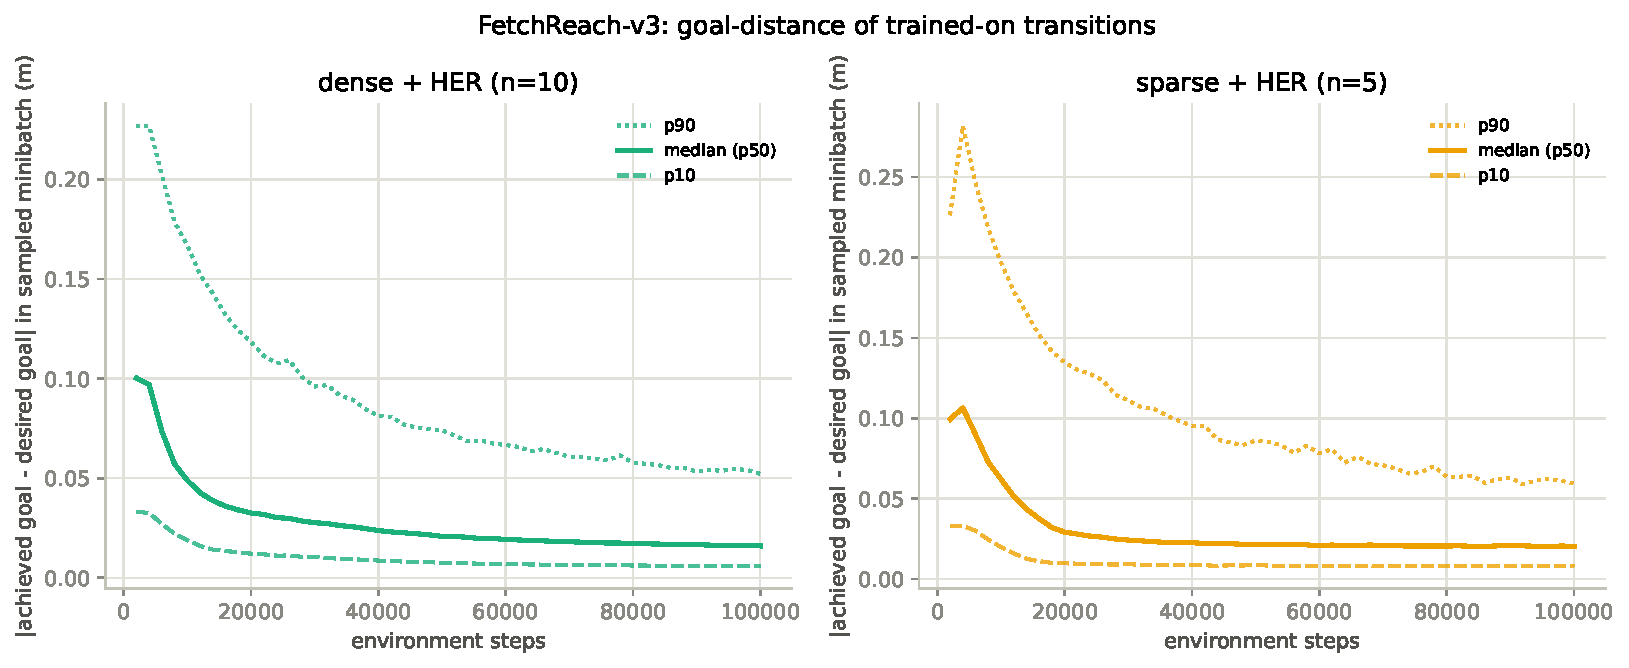
\includegraphics[width=\linewidth,height=4.3cm,keepaspectratio]{figures/fig5_reach_goal_distance.pdf}
\caption{FetchReach-v3 (dense+HER, sparse+HER)}
\end{subfigure}
\hfill
\begin{subfigure}{0.4\textwidth}
\centering
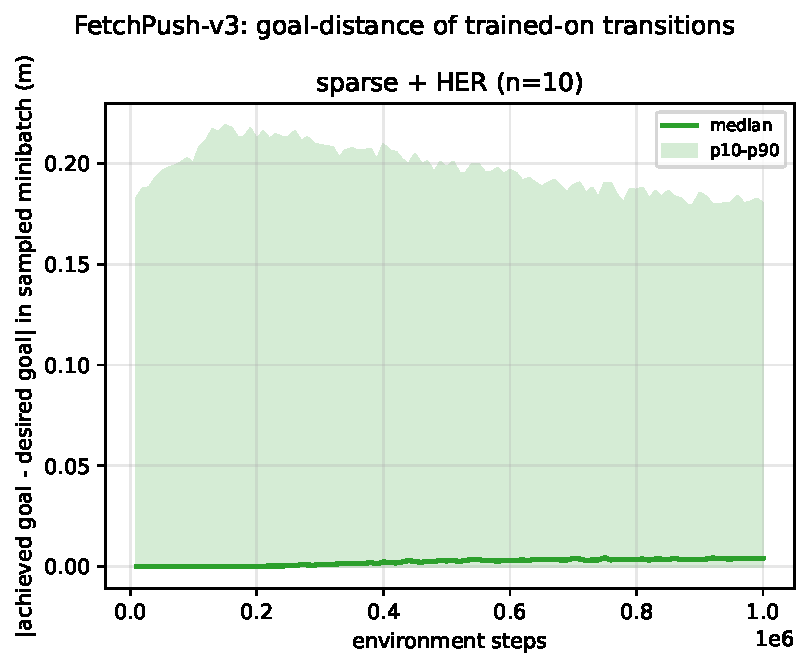
\includegraphics[width=\linewidth,height=4.3cm,keepaspectratio]{figures/fig5_push_goal_distance.pdf}
\caption{FetchPush-v3 (sparse+HER)}
\end{subfigure}
\caption{Median (line) and p10--p90 band of $\lVert$achieved $-$ desired
goal$\rVert$ across transitions actually sampled for training.}
\label{fig:curriculum}
\end{figure}

For the implicit-curriculum part of hypothesis (iii), the picture differs by
task. On Reach (Figure~\ref{fig:curriculum}a), the median trained-on goal
distance falls cleanly as training progresses --- from $\approx$0.10\,m to
$\approx$0.016--0.020\,m for dense+HER and sparse+HER respectively --- a
direct, visible curriculum: as the policy improves, the goals it is actually
trained on get closer on average. On Push (Figure~\ref{fig:curriculum}b) the
same signal is present but far less visible in this aggregate view: with
$n_{\text{sampled\_goal}}=4$, roughly 4 of every 5 stored transitions are
HER-relabeled (distance $\approx$0), which pins the median near zero for the
entire run and hides the curriculum in the remaining $\sim$20\% of
real-goal transitions. Those real-goal transitions do show a mild version of
the same effect --- the p10--p90 band widens from $\approx$0.18\,m to a peak
of $\approx$0.21--0.215\,m by $\sim$150--250k steps as the policy starts
reaching more diverse states, then narrows back to $\approx$0.18\,m by 1M
steps --- but it is a second-order effect on Push, not the dominant pattern
visible in the raw metric. We report this as an honest limitation of the
metric rather than evidence against hypothesis (iii): the entropy-coefficient
signal (Figure~\ref{fig:entropy}) is the clearer mechanism indicator on the
harder task.

\subsection{Ablation: does more relabeling always help?}

The proposal specifies this ablation over $n_{\text{sampled\_goal}} \in
\{1,4\}$, 5 seeds/setting; we additionally ran $n_{\text{sampled\_goal}}=8$
at the same 5 seeds/setting to check whether the trend continues past the
specified range.

\begin{table}[h]
\centering
\caption{HER relabeling-ratio ablation, FetchPush-v3 sparse+HER, 5 seeds/setting
(rows 1--4 are the specified range; row 8 is the extension).}
\label{tab:ablation}
\begin{tabular}{lcccc}
\toprule
$n_{\text{sampled\_goal}}$ & Final success & Seeds $\geq$90\% & Median steps to 90\% & AUC \\
\midrule
1 & 84.0\% & 4/5 & 400{,}000 & 0.566 \\
4 & 82.8\% & 4/5 & 380{,}000 & 0.553 \\
8 & 88.6\% & 4/5 & 260{,}000 & 0.637 \\
\bottomrule
\end{tabular}
\end{table}

\begin{figure}[h]
\centering
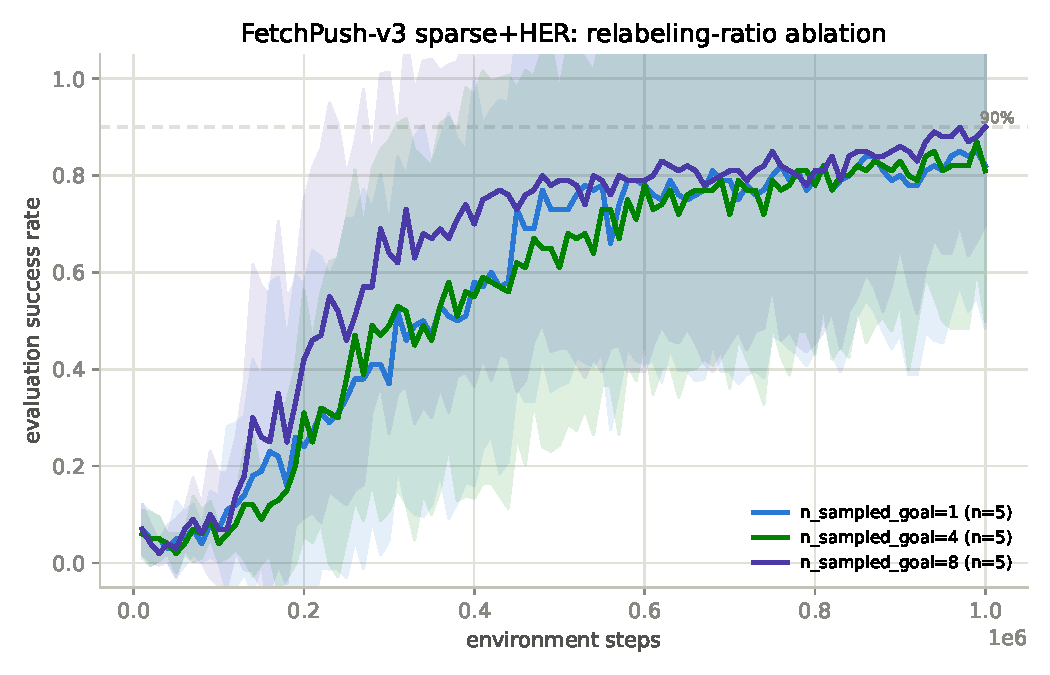
\includegraphics[width=0.65\textwidth]{figures/fig6_push_ablation.pdf}
\caption{Success rate by HER relabeling ratio on FetchPush-v3 (mean over 5
seeds, band: p10--p90).}
\label{fig:ablation}
\end{figure}

Table~\ref{tab:ablation} and Figure~\ref{fig:ablation} address the required
ablation: relabeling ratio does not help monotonically or dramatically.
$n_{\text{sampled\_goal}}=8$ learns somewhat faster (median steps-to-90\%
260{,}000 vs.\ $\sim$380--400{,}000) and reaches a marginally higher final
success and AUC, but $n_{\text{sampled\_goal}}=1$ and $4$ are statistically
indistinguishable from each other, and all three settings converge to a
similar success region by 1M steps. Every setting also has exactly one
seed out of five that fails to reach 90\% (final success 0.20--0.45 for that
seed, vs.\ $\geq$0.96 for the other four in the same group; visible as the
wide lower band in Figure~\ref{fig:ablation}) --- suggesting per-seed
optimization instability on this harder task is a bigger source of variance
than the relabeling ratio itself. We conclude the benefit of more relabeling
saturates quickly on this task rather than scaling with $k$.

\section{Discussion and Limitations}
The central result --- HER's benefit growing from a modest speedup on
FetchReach to the difference between learning and not learning on
FetchPush --- matches all three hypotheses from the proposal, and the
entropy-coefficient trajectories (Section~\ref{sec:mechanism}) give a
concrete mechanistic account of \emph{why}: HER prevents the premature,
overconfident entropy collapse that plain sparse-reward SAC falls into when
it never observes a success. We note three limitations. First, both
FetchPush conditions show occasional catastrophic-failure seeds (final
success as low as 0.20 despite HER); with only 10 (main grid) or 5
(ablation) seeds per setting, these outliers noticeably affect the mean and
should be reported alongside the median in any follow-up. Second, the
goal-distance curriculum signal, clear on Reach, is largely masked on Push by
the relabeling ratio itself (Section~\ref{sec:mechanism}); a cleaner
mechanism metric for harder tasks would track only the non-relabeled
("real-goal") transitions directly rather than the pooled distribution.
Third, we deviated from the proposal's literal evaluation cadence (every
2{,}000 steps) on Push, using 10{,}000 steps instead to keep evaluation
overhead proportionate to the $10\times$ longer training budget; this does
not affect the reported metrics' correctness but is a departure from the
originally specified protocol worth flagging explicitly.

\section{Reproducibility}
All code, trained checkpoints, logs, and this report's source are in the
project repository (see title page link). \texttt{README.md} documents the
software stack (pinned for the \texttt{gymnasium-robotics} 1.3.x /
\texttt{-v3} environments) and exact commands to reproduce every run;
\texttt{EXPERIMENT\_LOG.md} records the full chronological history of
decisions, calibration numbers, and cluster job IDs behind the numbers in
this report. \texttt{plot\_results.py} regenerates all figures and summary
tables in this report directly from \texttt{runs/}.

\section{Conclusion}
Across 70 training runs on two tasks of differing difficulty, HER's
contribution to SAC under sparse rewards is not fixed: it is a modest
accelerant on an easy task and the difference between success and failure on
a harder one, and this shift is traceable to HER sustaining healthy
exploration (via SAC's entropy coefficient) where plain sparse rewards let
the policy converge prematurely on a failing behavior. More hindsight
relabeling helps up to a point but saturates quickly, making
$n_{\text{sampled\_goal}}=4$--$8$ a reasonable default rather than a setting
worth aggressively tuning further.

\begin{thebibliography}{9}
\bibitem{haarnoja18}
T.~Haarnoja, A.~Zhou, P.~Abbeel, S.~Levine.
\newblock Soft Actor-Critic: Off-Policy Maximum Entropy Deep Reinforcement
Learning with a Stochastic Actor.
\newblock \emph{ICML}, 2018.

\bibitem{andrychowicz17}
M.~Andrychowicz, F.~Wolski, A.~Ray, J.~Schneider, R.~Fong, P.~Welinder,
B.~McGrew, J.~Tobin, P.~Abbeel, W.~Zaremba.
\newblock Hindsight Experience Replay.
\newblock \emph{NeurIPS}, 2017.

\bibitem{plappert18}
M.~Plappert, M.~Andrychowicz, A.~Ray, B.~McGrew, B.~Baker, G.~Powell,
J.~Schneider, J.~Tobin, M.~Chociej, P.~Welinder, V.~Kumar, W.~Zaremba.
\newblock Multi-Goal Reinforcement Learning: Challenging Robotics Environments
and Request for Research.
\newblock \emph{arXiv:1802.09464}, 2018.

\bibitem{schaul15}
T.~Schaul, D.~Horgan, K.~Gregor, D.~Silver.
\newblock Universal Value Function Approximators.
\newblock \emph{ICML}, 2015.

\bibitem{raffin20zoo}
A.~Raffin.
\newblock RL Baselines3 Zoo: A Training Framework for Stable-Baselines3
Reinforcement Learning Agents.
\newblock \url{https://github.com/DLR-RM/rl-baselines3-zoo}, 2020.

\bibitem{raffin21sb3}
A.~Raffin, A.~Hill, A.~Gleave, A.~Kanervisto, M.~Ernestus, N.~Dormann.
\newblock Stable-Baselines3: Reliable Reinforcement Learning Implementations.
\newblock \emph{JMLR}, 22(268), 2021.
\end{thebibliography}

\end{document}
